\section{LLM Implementation on a CGLA}
\label{proposed}

\begin{figure}[t]
  \centering
  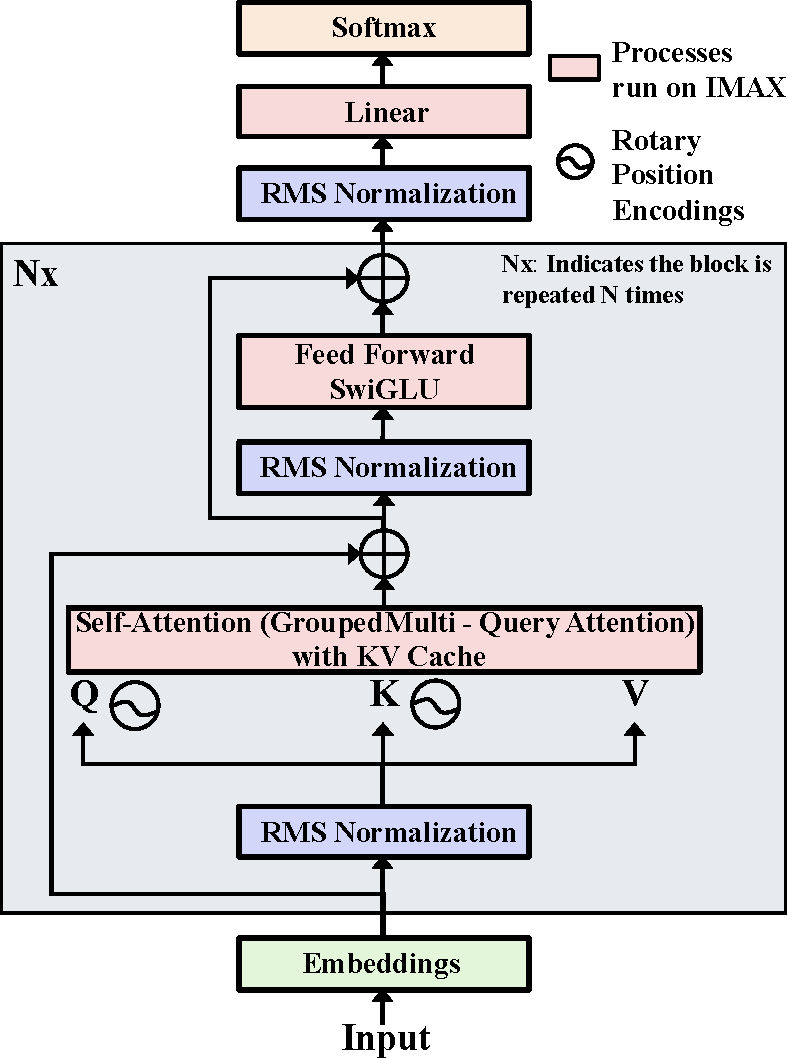
\includegraphics[width=0.95\columnwidth]{./llama_arch.pdf}
  \caption{Overview of the LLM inference architecture, based on the llama.cpp framework, and our proposed task partitioning.}
  \label{fig:llama_arch}
\end{figure}


\begin{figure*}[t]
  \centering
  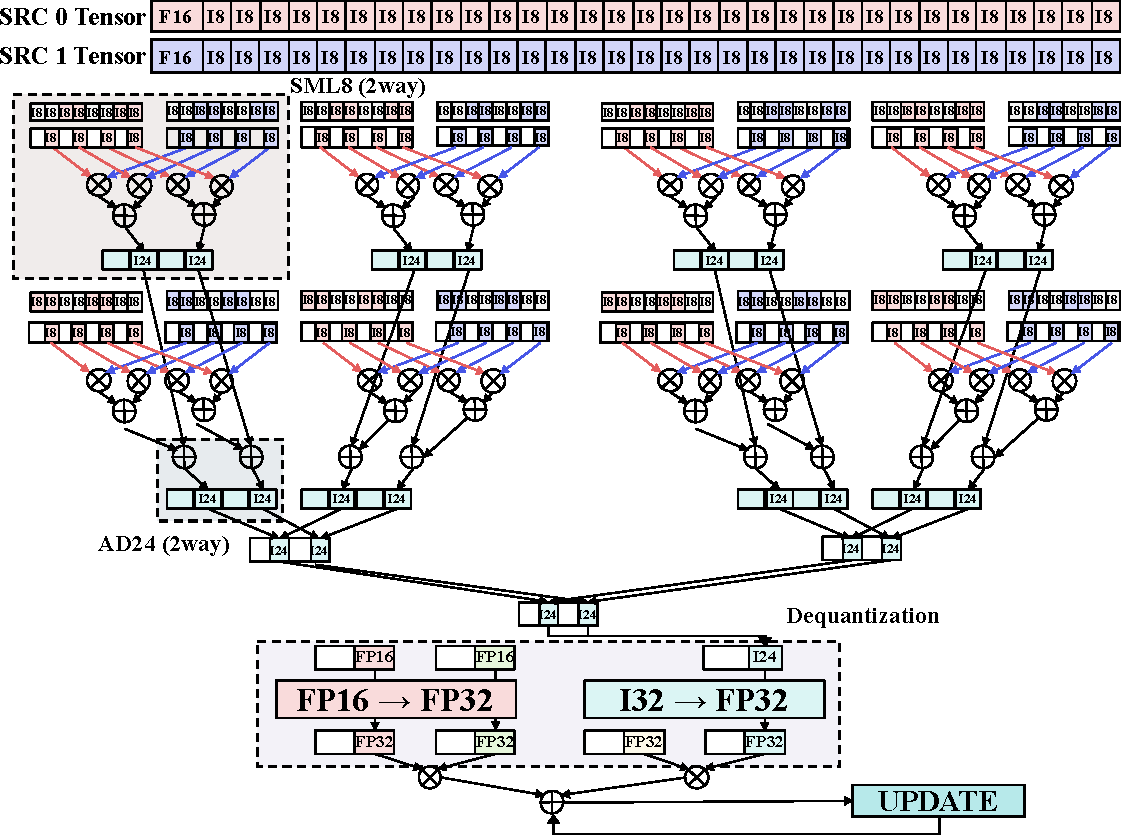
\includegraphics[width=1.85\columnwidth]{./q8dot.pdf}
  \caption{Detailed dataflow diagram for the parallelized Q8\_0 dot-product operation. This kernel uses parallel SML8 and AD24 custom instructions to perform the dot-product operation.}
  \label{fig:q8dot}
  \end{figure*}
  
  
  \begin{figure}[t]
  \centering
  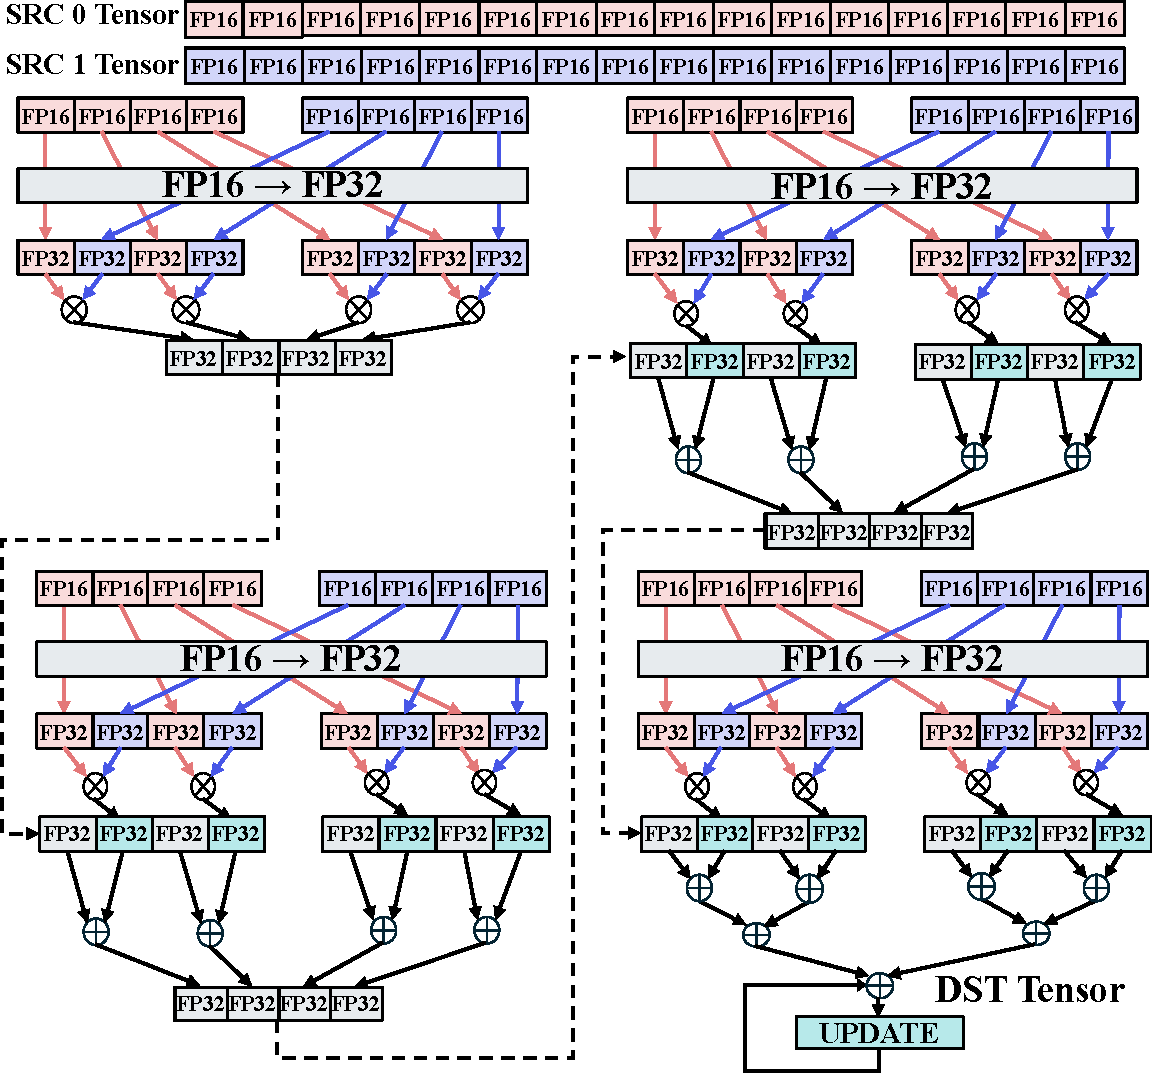
\includegraphics[width=0.95\columnwidth]{./f16dot.pdf}
  \caption{Detailed dataflow diagram for the parallelized FP16 dot-product operation as mapped onto the IMAX architecture.}
  \label{fig:f16dot}
  \end{figure}
This section details our methodology for implementing a recent LLM family, Qwen3, on IMAX, our general-purpose CGLA accelerator. 
We constructed a hybrid execution model built upon the widely adopted llama.cpp framework, which offloads computationally intensive kernels to the IMAX accelerator. 
We first provide an overview of the overall execution framework, followed by a detailed description of the dataflow design and mapping strategies for the various quantized kernels we implemented in this work.


\subsection{Execution Models and Framework Overview}
For a realistic system-level evaluation, we implement a hybrid execution model based on the llama.cpp framework.
For our target models, we selected the state-of-the-art Qwen3. 
We selected the Qwen3 for its high performance at smaller scales and its wide range of model sizes (e.g., 0.6B, 1.7B, 8B). 
This allows us to test our accelerator's capabilities on workloads ranging from edge to high-performance scenarios.
In our model, the host CPU and the IMAX accelerator collaborate on LLM inference.
Fig.~\ref{fig:llama_arch} presents a high-level view of the target LLM architecture and delineates our proposed task partitioning.
This partitioning is guided by the principle of assigning tasks to the most suitable processing unit: utilizing the CPU for complex, sequential control flow and the IMAX accelerator for parallel, computationally intensive operations.
The host CPU handles tasks that demand complex control and sequential logic. 
These responsibilities include prompt tokenization, embedding layer computations, KV cache management, and the final Softmax operation. 
Conversely, we offload the most computationally demanding kernels, which constitute the majority of the inference latency, to the IMAX accelerator. 
As highlighted in pink in Fig.~\ref{fig:llama_arch}, IMAX executes the dot-product operations within all linear projections, the Grouped Multi-Query Attention mechanism, and the linear transformations of the SwiGLU network. 
We retain non-linear operations, such as RMS Normalization and the application of Rotary Position Encodings, on the host CPU. 
We designed this functional partitioning to maximize overall system throughput by utilizing the architectural strengths of each processing unit.



\subsection{Quantization and Supported Kernels}
Quantization is an essential technique in LLM inference. 
It reduces both the memory footprint and the required memory bandwidth, while also enabling faster computation through integer arithmetic. 
In resource-constrained environments, model compression via quantization is often a prerequisite for execution. 
The llama.cpp framework supports a diverse range of quantization schemes, offering flexibility to balance the trade-off between model accuracy and performance.

To demonstrate the versatility and robustness of the IMAX architecture, we implemented and evaluated the following four distinct computational kernels, each with varying characteristics:
\begin{itemize}
    \item \textbf{FP16}: A \SI[number-unit-product=\nobreakdash-]{16}{bit} floating-point format. This serves not only as a baseline but is also an essential data type used for specific high-precision operations within all quantized models.
    \item \textbf{Q8\_0}: A standard \SI[number-unit-product=\nobreakdash-]{8}{bit} integer quantization scheme. This kernel constitutes the majority of the operations performed in the Q8\_0 models.
    \item \textbf{Q3\_K}: A highly compressed mixed-precision scheme by combining \SI[number-unit-product=\nobreakdash-]{1}{bit}, \SI[number-unit-product=\nobreakdash-]{2}{bit}, \SI[number-unit-product=\nobreakdash-]{4}{bit}, and \SI[number-unit-product=\nobreakdash-]{6}{bit} quantization blocks. It represents the majority of the computations in the highly compressed Q3\_K\_S models.
    \item \textbf{Q6\_K}: A \SI[number-unit-product=\nobreakdash-]{6}{bit} integer format that is also utilized for specific layers within the Q3\_K\_S models, complementing the Q3\_K kernel.
\end{itemize}

These data types are strategically employed across different layers of the models. 
The large weight matrices of the linear layers contain the majority of model parameters in the attention and feed-forward networks. 
These matrices are quantized to low-bit integer formats such as Q8\_0, Q3\_K, and Q6\_K.
This approach substantially reduces the overall model file size and memory bandwidth requirements. 
In contrast, we preserve the weights of the normalization layers in high-precision FP16 to avoid the risk of performance degradation, as these layers are necessary to maintain computational stability.
Since the parameter count in normalization layers is negligible compared to that of linear layers, retaining their precision has a minimal impact on the total model size. 
Our evaluation adopts a common strategy used in modern LLMs. 
We quantize only the large linear layers, while the smaller normalization layers remain in high precision to maintain model stability.

The selection of these specific quantization formats is intended to cover a realistic spectrum of quality-efficiency trade-offs. 
Empirical studies on the Qwen3 model family have demonstrated that \SI[number-unit-product=\nobreakdash-]{8}{bit} quantization (Q8\_0) maintains performance nearly identical to the FP16 baseline, with negligible degradation on standard benchmarks such as MMLU\cite{qwen3_quantization}. 
Conversely, quantization formats with extremely low bit-widths, such as Q3\_K, result in a measurable degradation in accuracy.
However, their reduced memory footprint, a \num{4.5}$\times$ reduction compared to FP16, makes them an enabling technology for deploying LLMs on severely memory-constrained edge devices. 
Our evaluation includes this range to demonstrate the architecture's flexibility across this entire spectrum.


  

\subsection{Kernel Mapping on IMAX}

% We map the dot-product operation for each data type onto the IMAX CGLA architecture using dedicated dataflows and custom instructions, designed to maximize pipelining and data-level parallelism. 
% In this subsection, we first describe the mapping of the FP16 kernel, which serves as our floating-point baseline. 
% We then detail the implementation of the Q8\_0 kernel, the foundation for all quantized operations, followed by the more complex mappings for the Q3\_K and Q6\_K mixed-precision kernels.

This section details how high-level dot-product operations from llama.cpp are compiled and mapped onto the IMAX CGLA architecture. 
The mapping process leverages IMAX's compiler-friendly design and a rich set of custom instructions to maximize pipelining and data-level parallelism.
First, the compiler analyzes the high-level C++ code, focusing on performance-critical loops such as the dot-product operation.
Then, it maps the dataflow of the operation onto IMAX's one-dimensional PE array. 
This linear topology, unlike 2D mesh architectures, allows for a deterministic mapping without complex routing heuristics, enabling predictable performance. 
Second, the compiler translates the low-level arithmetic within the dataflow into IMAX's custom instructions, which are designed to exploit fine-grained data parallelism as shown in Fig.~\ref{fig:q8dot}. 
The following subsections describe the specific dataflows and custom instructions used for each implemented kernel, serving as concrete examples of this mapping process.

Fig.~\ref{fig:f16dot} illustrates the dataflow for the FP16 dot-product kernel, which we designed to use the full programmability of IMAX. 
We first employ a lookup table (LUT) implemented within each PE to efficiently convert incoming FP16 data to an internal FP32 representation in-line, thus bypassing the need for dedicated conversion hardware. 
To enhance throughput, we then exploit two key parallelization features of IMAX. 
First, we apply SIMD instructions to execute two \SI[number-unit-product=\nobreakdash-]{32}{bit} operations concurrently on a single \SI[number-unit-product=\nobreakdash-]{64}{bit} datapath, maximizing the utilization of the Fused Multiply-Add (FMA) units. 
Second, we use column-wise multithreading to effectively mask the arithmetic pipeline latency. 
This technique time-multiplexes multiple logical FMA operations on a single physical FPU.
This kernel utilizes \num{22} arithmetic units to efficiently process a \num{16}-element multiplication in a single operational burst.




  
The dataflow for the Q8\_0 dot-product operation, shown in Fig.~\ref{fig:q8dot}, serves as the architectural foundation for all our quantized kernels. 
The IMAX dataflow efficiently integrates multiplication, addition, and data type conversion. 
We accelerate the core multiply-accumulate operation using the custom instructions conceptually illustrated in Fig.~\ref{fig:q8dot_one_unit}. 
The OP\_SML8 instruction performs a two-way SIMD signed \SI[number-unit-product=\nobreakdash-]{8}{bit} multiply-accumulate, independently multiplying each \SI[number-unit-product=\nobreakdash-]{8}{bit} segment of the input operands and summing the results into a sign-extended \SI[number-unit-product=\nobreakdash-]{24}{bit} output. 
We then use the OP\_AD24 instruction, a two-way \SI[number-unit-product=\nobreakdash-]{24}{bit} integer addition, to aggregate these intermediate results along the pipeline. 
Data is pipelined across twelve PEs and accumulated as \SI[number-unit-product=\nobreakdash-]{24}{bit} integers before being multiplied by a single-precision \SI[number-unit-product=\nobreakdash-]{32}{bit} floating-point scaling factor in the final stage. 
This entire process is replicated four times to run in parallel across the PE array, and two such parallel executions complete the processing of a full \num{32}\nobreakdash-element vector segment.
The Q8\_0 kernel utilizes a total of \num{46} arithmetic units.


\begin{figure}[t]
  \centering
  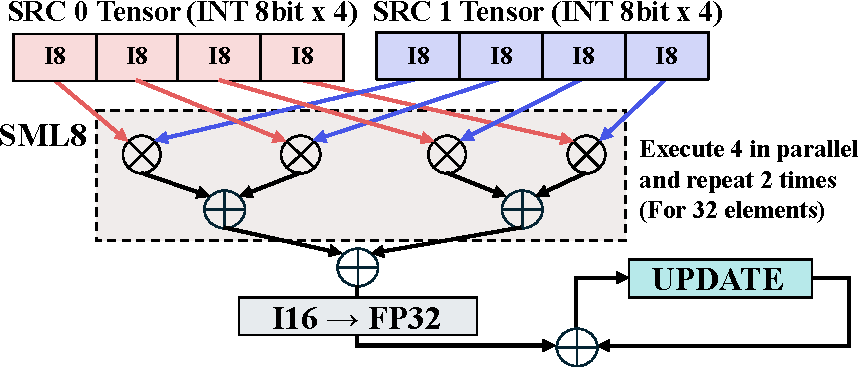
\includegraphics[width=0.95\columnwidth]{./q8dot_one_unit.pdf}
  \caption{Dataflow for the Q8\_0 dot-product operation with one unit. This kernel handles the 8-bit integer format.}
  \label{fig:q8dot_one_unit}
\end{figure}



\begin{figure}[t]
  \centering
  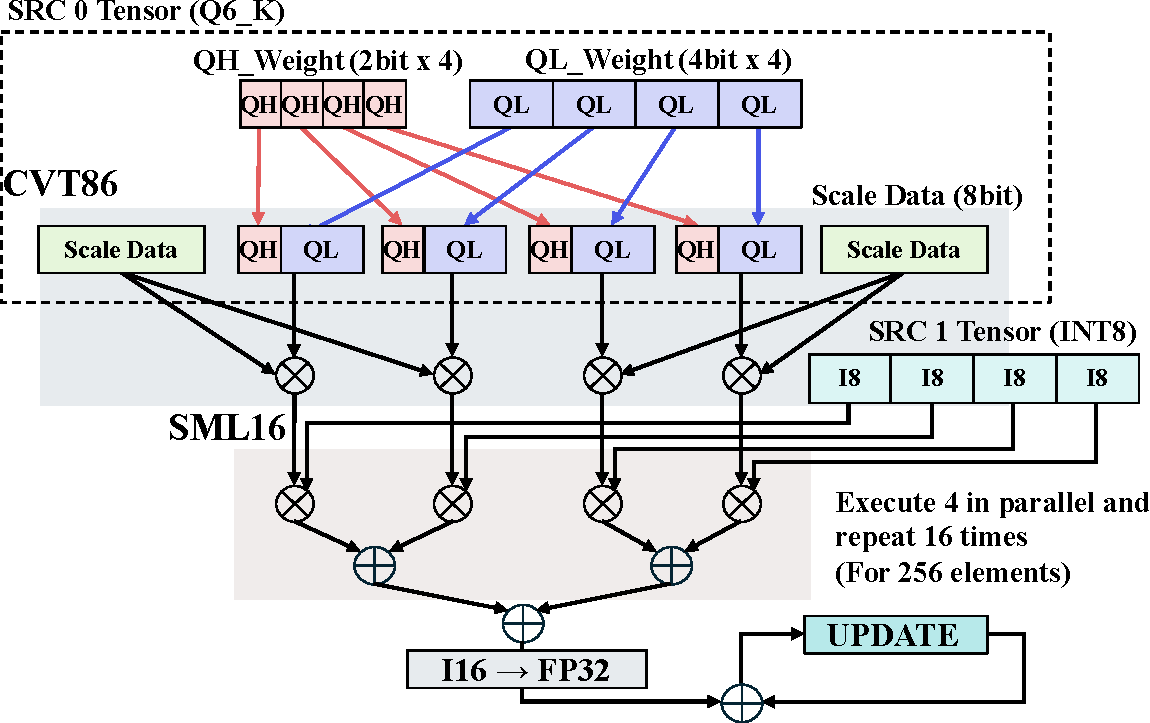
\includegraphics[width=0.95\columnwidth]{./q6kdot.pdf}
  \caption{Dataflow for the Q6\_K dot-product operation. This kernel handles the Q6\_K format, which packs 2-bit (QH) and 4-bit (QL) quantized weights.}

  \label{fig:q6kdot}
\end{figure}

\begin{figure}[t]
    \centering
    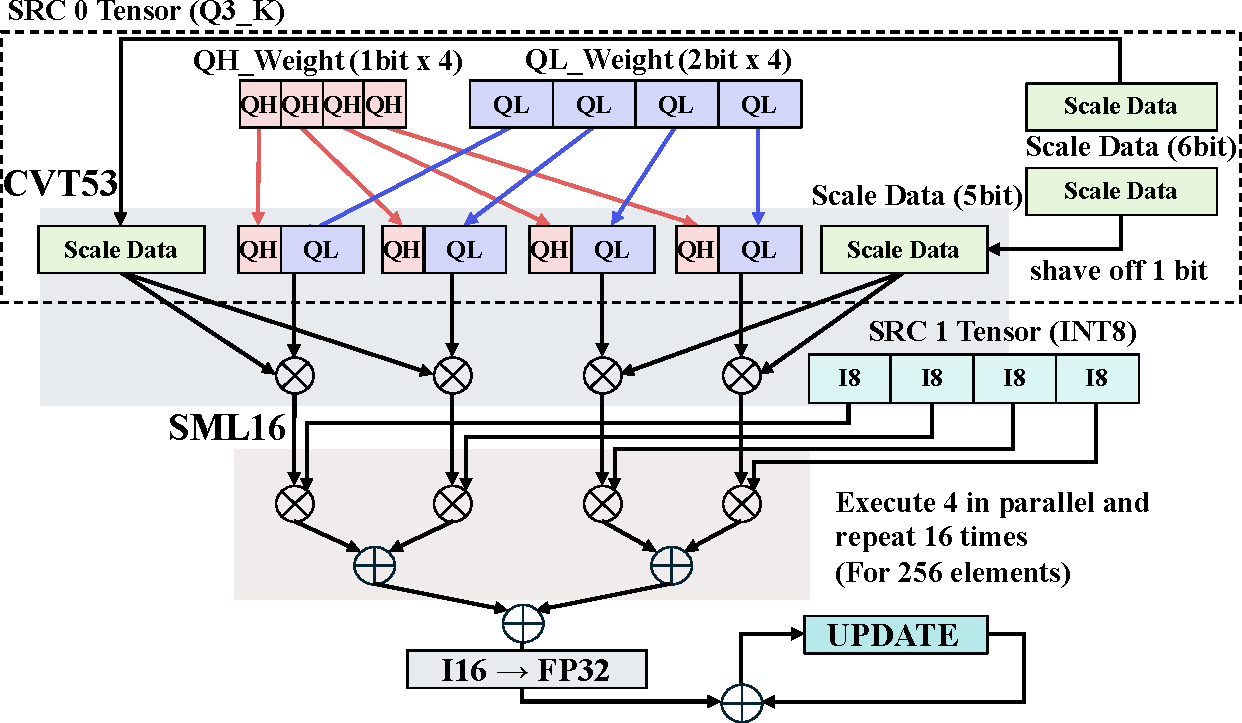
\includegraphics[width=0.95\columnwidth]{./q3kdot.pdf}
    \caption{Dataflow for the Q3\_K dot-product operation. This kernel handles the Q3\_K format, which packs 1-bit (QH) and 2-bit (QL) quantized weights.}
    \label{fig:q3kdot}
  \end{figure}
  
The dataflows for the Q6\_K and Q3\_K dot-product kernels, shown in Fig.~\ref{fig:q6kdot} and Fig.~\ref{fig:q3kdot}, respectively, build upon this Q8\_0 foundation. 
Although these low-bit mixed-precision kernels involve more complex data structures, they adopt a unified processing flow to maintain architectural versatility. 
The core strategy is to decompress and reconfigure the diverse low-bit formats into a common \SI[number-unit-product=\nobreakdash-]{8}{bit} integer (INT8) representation at the front-end, allowing the standardized back-end multiply-accumulate pipeline to be reused without modification.
The Q6\_K kernel utilizes \num{64} arithmetic units. For this kernel, a custom CVT86 instruction decodes incoming \SI[number-unit-product=\nobreakdash-]{2}{bit} and \SI[number-unit-product=\nobreakdash-]{4}{bit} quantized weights and their corresponding \SI[number-unit-product=\nobreakdash-]{8}{bit} scales in a single cycle, producing \SI[number-unit-product=\nobreakdash-]{16}{bit} intermediate data. Another custom instruction, SML16, then performs the dot-product operation between this decoded data and the \SI[number-unit-product=\nobreakdash-]{8}{bit} integer inputs.
This sequential execution of decompression followed by computation is a methodical approach to managing complex, packed data formats within the CGLA architecture.
The Q3\_K kernel, which uses \num{51} arithmetic units, requires even more intricate data manipulation. 
This format natively uses \SI[number-unit-product=\nobreakdash-]{6}{bit} scales with \SI[number-unit-product=\nobreakdash-]{2}{bit} and \SI[number-unit-product=\nobreakdash-]{1}{bit} quantized weights. 
To process this data efficiently on IMAX's SIMD architecture, we designed a custom data reconfiguration method. 
A dedicated instruction, OP\_CVT53, performs an approximate conversion of the \SI[number-unit-product=\nobreakdash-]{6}{bit} scales to \SI[number-unit-product=\nobreakdash-]{5}{bit} and packs the \SI[number-unit-product=\nobreakdash-]{2}{bit} and \SI[number-unit-product=\nobreakdash-]{1}{bit} segments into a unified \SI[number-unit-product=\nobreakdash-]{3}{bit} format. 
This reconfiguration enables the combination of \SI[number-unit-product=\nobreakdash-]{8}{bit} input data with \SI[number-unit-product=\nobreakdash-]{5}{bit} and \SI[number-unit-product=\nobreakdash-]{3}{bit} weight data, allowing us to implement a processing flow similar to that of the Q8\_0 kernel. 
We empirically confirmed that this approximation of the scale data, which carries less information than the weights, has a negligible impact on the final computational accuracy. 
This front-end conversion approach allows us to achieve high performance without architectural versatility, processing \num{256} elements per burst by running four parallel dataflows for sixteen iterations.



  
\subsection{LMM Management and Configuration}



\begin{table*}[t]
  \centering
  % 表全体を 'threeparttable' 環境で囲み、注釈を管理します。
  \begin{threeparttable}
  
  \caption{Physical specifications and performance comparisons of various devices.}
  \label{tab:processor_comparison_annotated}
  
  % 表の本体
  % ここを rllrrrrrrL に変更することで、両端に「見えない」列を追加し、スペースを確保します。
  % r と L はそれぞれ右揃えと左揃えの列として機能しますが、内容は空になります。
  \begin{tabular}{@{} llrrrrrrr l @{}} % ここを変更: 最初の @{} の後に l を追加し、最後の r @{} の後に l を追加
    \toprule
    % --- ヘッダー行 ---
    \textbf{Device} & \textbf{CPU} & \textbf{Cores} & \textbf{Chip area} & \textbf{Process node} & \textbf{Frequency} & \textbf{Memory} & \textbf{Power}\tnote{c} \\
    & & & \textbf{(mm$^2$)} & \textbf{(nm)} & \textbf{(MHz)} & & \textbf{(W)} \\
    \midrule
 
    % --- データ行 (注釈マーカー \tnote{...} を追加) --- 
    \textbf{IMAX3 (Xilinx VPK180)} & Arm Cortex-A72 & 64\tnote{a} & - & 7 & 145 & \SI{8}{\giga\byte} + \SI{4}{\giga\byte} DDR4\tnote{b} & 180 \\
 
    \textbf{IMAX3 (\SI{28}{\nano\meter})} & - & 64\tnote{a} & 14.6 & 28 & 840 & - & 2.16 - 6.1 \\
 
    
    \textbf{NVIDIA RTX 4090} & Xeon W5-2455X & 16384 & 608 & 5 & 2520 & \SI{24}{\giga\byte} + \SI{4}{\giga\byte} DDR6 & 450 \\
    \textbf{NVIDIA GTX 1080 Ti} & Xeon W5-2455X & 3584 & 448 & 16 & 1582 & \SI{11}{\giga\byte} DDR5 & 250 \\
    \textbf{Jetson AGX Orin 32GB} & Arm Cortex-A78AE & 1792 & 200 & 8 & 930 & \SI{32}{\giga\byte} DDR5 & 60 \\
    \bottomrule
  \end{tabular}

 \begin{tablenotes}[para,flushleft]
   \item[a] The number of cores for IMAX3 refers to the number of PEs per lane. 
   \item[b] \SI{8}{\giga\byte} DDR4 for OS buffer and \SI{4}{\giga\byte} DDR4 for DMA buffer.
  \item[c] For IMAX3~(\SI{28}{\nano\meter}), the power consumption is estimated and varies depending on the kernels (FP16: \SI{2.16}{\watt}, Q8\_0: \SI{4.41}{\watt}, Q3\_K: \SI{4.88}{\watt}, Q6\_K: \SI{6.1}{\watt}), references for other devices are from Cortex-A72\nobreak\cite{Versal}, Jetson AGX Orin \SI{32}{\giga\byte} (most high performance mode)\nobreak\cite{nvidia_jetson_agx_orin}, NVIDIA GTX 1080 Ti\nobreak\cite{nvidia_1080ti}, NVIDIA RTX 4090\nobreak\cite{nvidia_4090}.
 \end{tablenotes}
  
   \end{threeparttable}
  \end{table*}  


Although the LMMs are configurable up to \SI{512}{K\byte}, we selected a size of \SI{64}{K\byte} for all evaluations in this work. 
We found this configuration to be a favorable compromise between power consumption and performance, as it is sufficient to accommodate the tensor sizes involved in the dot-product operations of the Qwen3 models we evaluated. 
We will provide a quantitative justification for this choice in the discussion in Section~\ref{discussion}.
Data transfers between the host and IMAX via DMA can become a significant performance bottleneck, particularly for large-scale models. 
To mitigate this, we implemented a transfer coalescing strategy to maximize DMA efficiency. 
A naive implementation would issue separate DMA transactions for each input tensor (e.g., activations, weights, and scaling factors), incurring substantial overhead from multiple transaction setups. 
Although these tensors may reside in non-contiguous memory locations, our approach aggregates them into a single, contiguous block in the host-side DMA buffer before initiating the transfer.
For instance, the Q8\_0 kernel requires four distinct input arrays. 
By arranging them contiguously, the IMAX DMA engine, which utilizes a shared address space, can load the entire data block into the LMMs with a single burst-transfer instruction. 
A similar coalescing strategy is applied when writing results back to the host. 
This method significantly improves data transfer efficiency by minimizing the overhead associated with issuing multiple DMA transactions.
A preliminary evaluation of this optimization confirmed its effectiveness, accelerating the LOAD phase by a factor of 1.2 and the DRAIN phase by a factor of 4.8 compared to the naive implementation, which is a non-coalesced approach. 
All results reported in Section~\ref{ex_and_re} utilize this optimized data transfer method, demonstrating the critical importance of such low-level optimizations in memory-bound LLM workloads.




